\section{Lifting energy-level degeneracy}

The Hamiltonian for the outer electron of an Hydrogen-like atom can be written as
\begin{align*}
    H = \frac{p^2}{2m} + V_\text{eff}, 
\end{align*}
where:
\begin{align*}
        V_\text{eff} = - \frac{e^2}{4 \pi \varepsilon_0 r} \qquad &\text{for the Hydrogen atoms;} \\
        V_\text{eff} = - \frac{Z_\text{eff} e^2}{4 \pi \varepsilon_0 }\left( \frac{1}{r} - \mathcal{C}(r)\right) 
    \qquad &\text{with $Z_\text{eff} = 1$ for the neutral alkali atoms} \\
    &\text{or $Z_\text{eff} = 2$ for single-charged alkali-earth ions.}
\end{align*}
The term $\mathcal{C}(r)$ is a corrective term which is relevant for lower $l$. 
The energy levels are 
\begin{align*}
    E_{n,l} &= - \frac{m_e e^4 Z_\text{eff}^2}{2 (4 \pi \varepsilon_0)^2 \hbar^2} \left( \frac{1}{n^2} + \tilde{\mathcal{C}}_{n,l}(r)\right) = \\
    & = -\frac{m_e c^2}{2} Z_\text{eff}^2 \underbrace{\left( \frac{e^2}{4 \pi \varepsilon_0 \hbar c}\right)^2}_{\alpha^2} \left( \frac{1}{n^2} +  \tilde{\mathcal{C}}_{n,l}(r) \right),
\end{align*}
where $Z_\text{eff}$ is the residual charge at the outer shell and $\alpha$ is the fine structure constant. From the last expression, one can notice that the degeneracy in $n$ and $l$ is resolved. Nevertheless in many applications it is useful to have complete resolved energy levels and to obtain this situation the quantum numbers $m$ and $s_z$ are taken into account. In particular, the effects studied to remove this degeneracy are two:
\begin{itemize}
    \item \textit{Spin-orbit coupling}: it is an effect already present in the studied atoms and it derives from the fine structure; 
    \item \textit{Zeeman effect}: it derives from the application of an external magnetic field. 
\end{itemize}


\subsection{Spin-orbit coupling}

%\begin{center}
%

\tikzset{every picture/.style={line width=0.75pt}} %set default line width to 0.75pt        

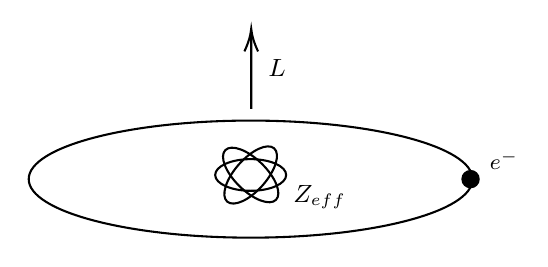
\begin{tikzpicture}[x=0.75pt,y=0.75pt,yscale=-1,xscale=1]
%uncomment if require: \path (0,125); %set diagram left start at 0, and has height of 125

%Flowchart: Connector [id:dp31225744112714693] 
\draw   (13.33,83.21) .. controls (13.33,67.63) and (61.21,55) .. (120.27,55) .. controls (179.32,55) and (227.2,67.63) .. (227.2,83.21) .. controls (227.2,98.78) and (179.32,111.41) .. (120.27,111.41) .. controls (61.21,111.41) and (13.33,98.78) .. (13.33,83.21) -- cycle ;
%Shape: Boxed Line [id:dp7490815418622135] 
\draw    (120.56,49.41) -- (120.53,12.74) ;
\draw [shift={(120.53,10.74)}, rotate = 89.96] [color={rgb, 255:red, 0; green, 0; blue, 0 }  ][line width=0.75]    (10.93,-3.29) .. controls (6.95,-1.4) and (3.31,-0.3) .. (0,0) .. controls (3.31,0.3) and (6.95,1.4) .. (10.93,3.29)   ;
%Shape: Circle [id:dp30161062782824144] 
\draw  [fill={rgb, 255:red, 0; green, 0; blue, 0 }  ,fill opacity=1 ] (222.27,83.21) .. controls (222.27,81.03) and (224.03,79.27) .. (226.2,79.27) .. controls (228.37,79.27) and (230.13,81.03) .. (230.13,83.21) .. controls (230.13,85.38) and (228.37,87.14) .. (226.2,87.14) .. controls (224.03,87.14) and (222.27,85.38) .. (222.27,83.21) -- cycle ;
%Shape: Ellipse [id:dp5616793906082976] 
\draw   (103.17,81.21) .. controls (103.17,76.99) and (110.82,73.58) .. (120.27,73.58) .. controls (129.71,73.58) and (137.37,76.99) .. (137.37,81.21) .. controls (137.37,85.42) and (129.71,88.83) .. (120.27,88.83) .. controls (110.82,88.83) and (103.17,85.42) .. (103.17,81.21) -- cycle ;
%Shape: Ellipse [id:dp7473632087803942] 
\draw   (108.95,94.03) .. controls (105.79,91.24) and (108.3,83.24) .. (114.55,76.16) .. controls (120.8,69.08) and (128.42,65.6) .. (131.58,68.38) .. controls (134.74,71.17) and (132.23,79.17) .. (125.98,86.25) .. controls (119.73,93.33) and (112.11,96.81) .. (108.95,94.03) -- cycle ;
%Shape: Ellipse [id:dp36775889518050264] 
\draw   (108.05,69.24) .. controls (111,66.23) and (118.86,69.15) .. (125.6,75.76) .. controls (132.35,82.37) and (135.43,90.17) .. (132.48,93.17) .. controls (129.53,96.18) and (121.68,93.26) .. (114.93,86.65) .. controls (108.18,80.04) and (105.11,72.24) .. (108.05,69.24) -- cycle ;

% Text Node
\draw (127.33,24.07) node [anchor=north west][inner sep=0.75pt]  [font=\small]  {$L$};
% Text Node
\draw (234,68.07) node [anchor=north west][inner sep=0.75pt]  [font=\footnotesize]  {$e^{-}$};
% Text Node
\draw (139.37,84.61) node [anchor=north west][inner sep=0.75pt]  [font=\small]  {$Z_{\text{eff}}$};


\end{tikzpicture}
%\end{center}

Consider the an Hydrogen-like atom in a laboratory frame in absence of magnetic fields and imagine that the outer electron moves with velocity $\vec{v}$. If the problem is studied from the frame in which the electron is at rest, the latter experiences an effective magnetic field
\begin{align}
    \vec{B}_{el} = -\frac{1}{c^2} \vec{v} \times \vec{E}, 
    \label{eq:B}
\end{align}
where $\vec{E}$ is the core electric field measured in the laboratory frame. Since $\vec{E}$ is radial, one can write 
\begin{align*}
    \vec{E} = \frac{\vec{\nabla}V}{e} = \frac{\vec{r}}{e {r}} \frac{\partial V_\text{eff}}{\partial r} , 
\end{align*}
while $\vec{v} = \vec{p}/m_e$ (in non-relativistic approximation). Therefore, equation (\ref{eq:B}) becomes
\begin{align}
    \vec{B}_{el} = -\frac{1}{c^2} \left( \frac{\vec{p}}{m_e} \times \vec{r} \right) \frac{1}{e {r}} \frac{\partial V_\text{eff} }{\partial r} = \frac{1}{e m_e c^2 r} \frac{\partial V_\text{eff}}{\partial r}  \vec{L}, 
\end{align}
where $\vec{L}$ is the angular momentum in the laboratory frame. \\

This magnetic field can couple with the magnetic dipole moment associated to the electron spin, given by 
\begin{align*}
    \vec{\mu}_s = -\frac{e}{2 m_e} g_s \vec{S} = -\mu_B g_s \vec{S},  
\end{align*}
where $g_s$ is the electron $g$-factor ($g_s = 2$ from Dirac free theory) and $\mu_B = e\hbar/(2 m_e)$ is the Bohr magneton. In particular, the additional term to the Hamiltonian of the electron evaluated in the electron reference frame is 
\begin{align}
    H_\text{spin-orbit}^{el} \equiv H_{SO}^{el} = - \vec{\mu}_s \cdot \vec{B}_{el} = \frac{\mu_B g_s}{e m c^2 \hbar} \left( \frac{1}{r} \frac{\partial V_\text{eff}}{\partial r} \right)\vec{S} \cdot \vec{L}. 
\end{align}
The following step consists of returning to the laboratory frame. The explicit calculation leads to the following terms 
\begin{align}
    H_\text{spin-orbit}^{lab} \equiv H_{SO}^{lab} = \frac{\mu_B (g_S-1)}{e m c^2 \hbar} \left( \frac{1}{r} \frac{\partial V_\text{eff}}{\partial r} \right)\vec{S} \cdot \vec{L}. 
\end{align}
Using the general expression for $V_\text{eff}$ presented above, the spin-orbit Hamiltonian is 
\begin{align}
    H_{SO}^{lab} = \frac{\mu_B (g_S-1)Z_\text{eff} e}{4 \pi \varepsilon_0 m c^2 \hbar} \left( \frac{1}{r^3} - \frac{\partial \mathcal{C}}{\partial r} \right) \vec{S} \cdot \vec{L}, 
\end{align}
or more in general (omitting the reference to the laboratory frame)
$$H_{SO} = \Bigl( \textrm{some function of } r\Bigr) \; \vec{L}\cdot\vec{S}.$$
The basis formed by elements like $\ket{l,m,s,s_z}$ does not diagonalize this Hamiltonian. In order to do this, one has to introduce the \textit{total angular momentum}
\begin{align}
    \vec{J} = \vec{L} + \vec{S} 
\end{align}
and the new useful basis becomes $\ket{l,s,j,j_z}$ (indeed $L^2$, $S^2$, $J^2$ and $J_z$ commute). Hence from 
\begin{align*}
    \begin{pmatrix}
    L^2 \\ L_z \\ S^2 \\ S_z 
    \end{pmatrix}
    \ket{l,m,s,s_z} = 
    \begin{pmatrix}
    \hbar^2 l(l+1) \\ \hbar m \\ \hbar^2 s(s+1) \\ \hbar s_z 
    \end{pmatrix}
    \ket{l,m,s,s_z} 
\end{align*}
one passes to 
\begin{align*}
    \begin{pmatrix}
    L^2 \\ S^2 \\ J^2 \\ J_z 
    \end{pmatrix}
    \ket{l,s,j,j_z} = 
    \begin{pmatrix}
    \hbar^2 l(l+1) \\ \hbar^2 s(s+1) \\  \hbar^2 j(j+1) \\ \ \hbar j_z 
    \end{pmatrix}
    \ket{l,s,j,j_z}
\end{align*}
with 
\begin{align*}
    j = l +\dfrac{1}{2}, l - \dfrac{1}{2} \qquad \text{and} \qquad j_z = -j, ..., j.
\end{align*}
In principle, one should evaluate the Clebsch-Gordan coefficient to move from one basis to another, but in this case a simpler approach is used. \\
The term $\vec{L} \cdot \vec{S}$ in $H_{SO}$ can be rewritten by noticing that
\begin{align*}
{J}^2 & = (\vec{L} + \vec{S})^2 = {S}^2 + {L}^2 + \vec{S}\cdot\vec{L} + \vec{L}\cdot\vec{S} = {S}^2 + {L}^2 + 2\vec{L}\cdot\vec{S},
\end{align*}
where the last equation is obtained from the fact that $\vec{L}$ and $\vec{S}$ commute because the operators act on different spaces. From this
\begin{equation*}
\vec{L}\cdot\vec{S} = \frac{1}{2}\left( {J}^2 - {L}^2 - {S}^2\right)
\end{equation*}
and hence 
\begin{align}
    H_{SO} \simeq \Bigl( \textrm{some function of } r\Bigr) \left( {J}^2 - {L}^2 - {S}^2\right), 
\end{align}
which is clearly diagonalized by $\ket{n,l,s,j,j_z}$. 

Once the new basis is found, the first-order degeneracy removing Hamiltonian is given by (\ref{eq:H1})
\begin{align*}
    H^{(1)} = \Pi_{n,l,s=1/2}\, H_{SO}  \, \Pi_{n,l,s=1/2} 
\end{align*}
while the associated energy shift is 
\begin{align*}
\Delta E_{{SO}}^{(1)} & = \bra{n,l,j,j_z} H_{SO} \ket{n,l,j,j_z} = \\
& \propto   \underbrace{ \bra{n,l}{\left( \frac{1}{r}\frac{\partial V_{\text{eff}}}{\partial r} \right)}\ket{n,l} }_{\text{just an integral $>$ 0}}  \left( j(j+1) - l(l+1) - \underbrace{s(s+1)}_{3/4} \right)
\end{align*}
This expression shows that some degeneracies are removed, as levels with same $l$ are now split by means of $j = l \pm \frac{1}{2}$. 
\begin{center}


\tikzset{every picture/.style={line width=0.75pt}} %set default line width to 0.75pt        

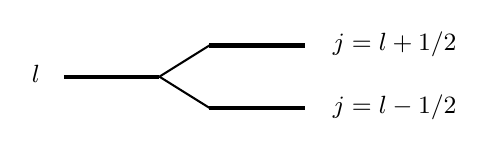
\begin{tikzpicture}[x=0.75pt,y=0.75pt,yscale=-1,xscale=1]
%uncomment if require: \path (0,84); %set diagram left start at 0, and has height of 84

%Straight Lines [id:da5451741662949235] 
\draw [line width=1.5]    (30,45) -- (75.97,45) ;
%Straight Lines [id:da037325881742858114] 
\draw [line width=1.5]    (100,30) -- (107.37,30) -- (145.97,30) ;
%Straight Lines [id:da1983425953314939] 
\draw [line width=1.5]    (100,60) -- (145.97,60) ;
%Straight Lines [id:da734262702937892] 
\draw    (75.97,45) -- (100,30) ;
%Straight Lines [id:da9010281726737945] 
\draw    (75.97,45) -- (100,60) ;

% Text Node
\draw (13,37.9) node [anchor=north west][inner sep=0.75pt]  [font=\small]  {$l$};
% Text Node
\draw (158,21.9) node [anchor=north west][inner sep=0.75pt]  [font=\small]  {$j=l+1/2$};
% Text Node
\draw (158,52.4) node [anchor=north west][inner sep=0.75pt]  [font=\small]  {$j=l-1/2$};


\end{tikzpicture}

\end{center}

A final note is about the fact that in this procedure the relativistic effects are neglected. Nevertheless, they do not determine, at this level, a splitting but a shift of all energy levels of the order of $2\pi/\alpha^2$. 


\begin{tcolorbox} [breakable, enhanced]
\textbf{Note about notation}\\ 
A state with quantum numbers $n, l, s, j$ is labelled as $$n^{2s+1}l_j$$
where $l$ is replaced with a capital letter according to its value. The first four values are associated to: 
\begin{align*}
l=0 \rightarrow S \qquad & l=1 \rightarrow P\\
l=2 \rightarrow D \qquad & l=3 \rightarrow F 
\end{align*}
For instance, $4^2S_{1/2}  \Longleftrightarrow \ket{n=4,l=0,s=1/2,j=1/2}$.
\end{tcolorbox}

\begin{tcolorbox} [breakable, enhanced]
\textbf{Fine structure of Sodium} ($Z=11$) \\
A partial lifting of the degeneracy in Sodium spectrum is reported below. The energy levels $3^2 P_{1/2}$ and $3^2 P_{3/2}$ are two-time and four-time degenerate, hence the degeneracy is only partially removed. 
\begin{center}


\tikzset{every picture/.style={line width=0.75pt}} %set default line width to 0.75pt        

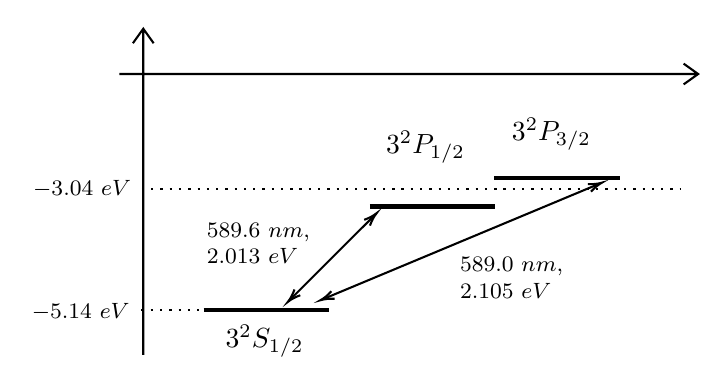
\begin{tikzpicture}[x=0.75pt,y=0.75pt,yscale=-1,xscale=1]
%uncomment if require: \path (0,182); %set diagram left start at 0, and has height of 182

%Shape: Axis 2D [id:dp3017160538012129] 
\draw  (45.33,32.16) -- (324.2,32.16)(56.87,10.33) -- (56.87,167.43) (317.2,27.16) -- (324.2,32.16) -- (317.2,37.16) (51.87,17.33) -- (56.87,10.33) -- (61.87,17.33)  ;
%Straight Lines [id:da24085599967696059] 
\draw [line width=1.5]    (86,146) -- (146.47,146) ;
%Straight Lines [id:da1539316269981591] 
\draw [line width=1.5]    (166,96) -- (226.47,96) ;
%Straight Lines [id:da40743469547233857] 
\draw [line width=1.5]    (226,82.33) -- (286.47,82.33) ;
%Straight Lines [id:da6604133921274191] 
\draw  [dash pattern={on 0.84pt off 2.51pt}]  (56.2,87.67) -- (315.53,87.67) ;
%Straight Lines [id:da1648566831794681] 
\draw  [dash pattern={on 0.84pt off 2.51pt}]  (56,146) -- (86,146) ;
%Straight Lines [id:da12556235022798856] 
\draw    (167.92,100.57) -- (127.88,140.59) ;
\draw [shift={(126.47,142)}, rotate = 315.01] [color={rgb, 255:red, 0; green, 0; blue, 0 }  ][line width=0.75]    (6.56,-1.97) .. controls (4.17,-0.84) and (1.99,-0.18) .. (0,0) .. controls (1.99,0.18) and (4.17,0.84) .. (6.56,1.97)   ;
\draw [shift={(169.33,99.16)}, rotate = 135.01] [color={rgb, 255:red, 0; green, 0; blue, 0 }  ][line width=0.75]    (6.56,-1.97) .. controls (4.17,-0.84) and (1.99,-0.18) .. (0,0) .. controls (1.99,0.18) and (4.17,0.84) .. (6.56,1.97)   ;
%Straight Lines [id:da5918618746875237] 
\draw    (276.02,85.26) -- (144.05,140.38) ;
\draw [shift={(142.2,141.16)}, rotate = 337.33] [color={rgb, 255:red, 0; green, 0; blue, 0 }  ][line width=0.75]    (6.56,-1.97) .. controls (4.17,-0.84) and (1.99,-0.18) .. (0,0) .. controls (1.99,0.18) and (4.17,0.84) .. (6.56,1.97)   ;
\draw [shift={(277.87,84.49)}, rotate = 157.33] [color={rgb, 255:red, 0; green, 0; blue, 0 }  ][line width=0.75]    (6.56,-1.97) .. controls (4.17,-0.84) and (1.99,-0.18) .. (0,0) .. controls (1.99,0.18) and (4.17,0.84) .. (6.56,1.97)   ;

% Text Node
\draw (95,151.4) node [anchor=north west][inner sep=0.75pt]    {$3^{2} S_{1/2}$};
% Text Node
\draw (172.33,58.07) node [anchor=north west][inner sep=0.75pt]    {$3^{2} P_{1/2}$};
% Text Node
\draw (233,52.07) node [anchor=north west][inner sep=0.75pt]    {$3^{2} P_{3/2}$};
% Text Node
\draw (2.33,82.07) node [anchor=north west][inner sep=0.75pt]  [font=\footnotesize]  {$-3.04\ eV$};
% Text Node
\draw (1.67,141.07) node [anchor=north west][inner sep=0.75pt]  [font=\footnotesize]  {$-5.14\ eV$};
% Text Node
\draw (201.33,117.07) node [anchor=north west][inner sep=0.75pt]  [font=\footnotesize]  %{$589.0\ nm,\ 2.105\ eV$};
{$ \begin{array}{l}
589.0\ nm,\\
2.105\ eV
\end{array}$};
% Text Node
\draw (79.33,100.4) node [anchor=north west][inner sep=0.75pt]  [font=\footnotesize]  {$ \begin{array}{l}
589.6\ nm,\\
2.013\ eV
\end{array}$};


\end{tikzpicture}

\end{center}
\end{tcolorbox}

From the Sodium example it is evident that, to have a complete resolution of the energy levels, something different must be introduced. 

\subsection{Zeeman effect}

Consider the system described in the previous section with an external classical magnetic field $\vec{B}$. The interaction is described by the Hamiltonian
\begin{equation*}
H_B = -\vec{\mu}_s\cdot \vec{B} -\vec{\mu}_l\cdot \vec{B} = \frac{\mu_B}{\hbar} \left( g_s \vec{S} + g_l \vec{L}\right) \cdot \vec{B}
\label{eq:HB}
\end{equation*}
where
\begin{equation*}
g_s \simeq 2.0023 \qquad \text{and} \qquad g_l \simeq \frac{m_{\textrm{reduced}}}{m_{e^-}} = \frac{1}{1 + m_e/m_\text{reduced}}\lesssim 1
\end{equation*}
are the electron spin $g$-factor and the orbital $g$-factor respectively. 
In (\ref{eq:HB}), $\vec{\mu}_s$ is the spin magnetic dipole moment while $\vec{\mu}_l$ is the orbital magnetic dipole moment. 

To simplify even more, one can orient $\vec B$ along the $\vec{z}$ axis and hence 
\begin{equation*}
H_B = \frac{\mu_B}{\hbar} \left( 2S_z + L_z \right) B_z
\end{equation*} 


\subsubsection{Case 1: Strong $\vec B$ regime}

By ``strong $B$ regime" one refers to a situation in which the energies associated to the magnetic field are much bigger than those of spin-orbit, namely $\Delta E_B \gg \Delta E_{SO}$.

In this case, $n,l,m$ and $s_z$ are good quantum numbers and the computation of the energy shift is straightforward:
\begin{align*}
\Delta E_{n,l,m,s_z} &= \bra{n,l,m,s_z} H_B \ket{n,l,m,s_z} =\\
& = \frac{\mu_B B}{\hbar} \bra{n,l,m,s_z}  2S_z + L_z \ket{n,l,m,s_z} = \mu_B (2s_z + m)B
\end{align*}
In this regime, the splitting is called \textit{Paschen-Back effect}.

\begin{tcolorbox} [breakable, enhanced]
\textbf{Paschen-Back effect for a $P$ level}
\begin{center}
\tikzset{every picture/.style={line width=0.75pt}} %set default line width to 0.75pt        

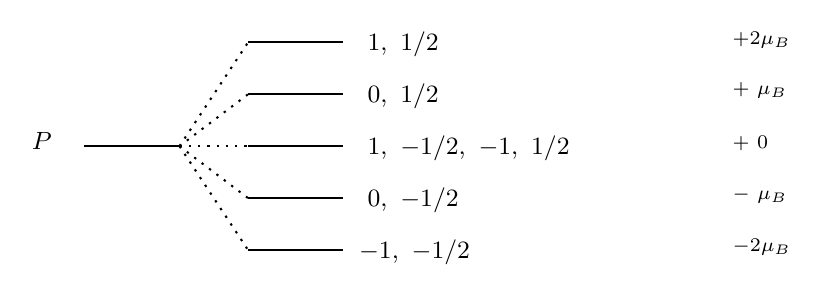
\begin{tikzpicture}[x=0.75pt,y=0.75pt,yscale=-1,xscale=1]
%uncomment if require: \path (0,141); %set diagram left start at 0, and has height of 141

%Straight Lines [id:da8975336306251028] 
\draw    (41,70) -- (56.97,70) -- (86.97,70) ;
%Straight Lines [id:da28508596950100773] 
\draw [line width=0.75]    (120,20) -- (135.97,20) -- (165.97,20) ;
%Straight Lines [id:da44121474273875605] 
\draw [line width=0.75]    (120,45) -- (135.97,45) -- (165.97,45) ;
%Straight Lines [id:da8891350329962026] 
\draw [line width=0.75]    (120,70) -- (135.97,70) -- (165.97,70) ;
%Straight Lines [id:da31409125050054265] 
\draw [line width=0.75]    (120,95) -- (135.97,95) -- (165.97,95) ;
%Straight Lines [id:da3078724766520293] 
\draw [line width=0.75]    (120,120) -- (135.97,120) -- (165.97,120) ;
%Straight Lines [id:da21353385953707116] 
\draw  [dash pattern={on 0.84pt off 2.51pt}]  (86.97,70) -- (120,20) ;
%Straight Lines [id:da2989866705363874] 
\draw  [dash pattern={on 0.84pt off 2.51pt}]  (86.97,70) -- (120,120) ;
%Straight Lines [id:da6705557415835165] 
\draw  [dash pattern={on 0.84pt off 2.51pt}]  (86.97,70) -- (120,95) ;
%Straight Lines [id:da2096870206528575] 
\draw  [dash pattern={on 0.84pt off 2.51pt}]  (86.97,70) -- (120,70) ;
%Straight Lines [id:da22004352286960305] 
\draw  [dash pattern={on 0.84pt off 2.51pt}]  (86.97,70) -- (120,45) ;

% Text Node
\draw (14.33,62.07) node [anchor=north west][inner sep=0.75pt]  [font=\small]  {$P$};
% Text Node
\draw (172,13.4) node [anchor=north west][inner sep=0.75pt]  [font=\small]  {$\ket{\ 1,\ 1/2}$};
% Text Node
\draw (172,38.4) node [anchor=north west][inner sep=0.75pt]  [font=\small]  {$\ket{\ 0,\ 1/2}$};
% Text Node
\draw (172,63.4) node [anchor=north west][inner sep=0.75pt]  [font=\small]  {$\ket{\ 1,\ -1/2} ,\ \ket{-1,\ 1/2}$};
% Text Node
\draw (172,88.4) node [anchor=north west][inner sep=0.75pt]  [font=\small]  {$\ket{\ 0,\ -1/2}$};
% Text Node
\draw (172,113.4) node [anchor=north west][inner sep=0.75pt]  [font=\small]  {$\ket{-1,\ -1/2}$};
% Text Node
\draw (352,13.4) node [anchor=north west][inner sep=0.75pt]  [font=\scriptsize]  {$+2\mu _{B}$};
% Text Node
\draw (352,37.73) node [anchor=north west][inner sep=0.75pt]  [font=\scriptsize]  {$+\ \mu _{B}$};
% Text Node
\draw (352,63.4) node [anchor=north west][inner sep=0.75pt]  [font=\scriptsize]  {$+\ 0\ $};
% Text Node
\draw (352,88.4) node [anchor=north west][inner sep=0.75pt]  [font=\scriptsize]  {$-\ \mu _{B}$};
% Text Node
\draw (352,113.4) node [anchor=north west][inner sep=0.75pt]  [font=\scriptsize]  {$-2\mu _{B}$};


\end{tikzpicture}

\end{center}

The degeneracy of $\ket{m,s_z} = \ket{1, -1/2}, \ket{-1, 1/2}$ is eventually removed by relativistic effects.
\end{tcolorbox}

\subsubsection{Case 2: Weak $\vec B$ regime}

On the other hand, one might consider the range of energies in which $\Delta E_B \lesssim \Delta E_{SO}$; in this case, the quantum numbers $n,l,j$ and $j_z$ are used:
\begin{align*}
\Delta E_{n,l,j,j_z} & = \bra{n,l,j,j_z} H_B \ket{n,l,j,j_z} =\\
& = \frac{\mu_B B}{\hbar} \bra{n,l,j,j_z} g_sS_z + g_lL_z \ket{n,l,j,j_z} = \\
& = \frac{\mu_B B}{\hbar} \bra{n,l,j,j_z}  (g_s-g_l)S_z + g_lJ_z \ket{n,l,j,j_z} = \\
&= \frac{\mu_B B}{\hbar} \bigg[ (g_s-g_l)\bra{n,l,j,j_z}S_z\ket{n,l,j,j_z} + g_l\hbar j_z \bigg]
\end{align*}
From the last line, one notices that there is not a straightforward way to evaluate $\bra{n,l,j,j_z}S_z\ket{n,l,j,j_z}$ no eigenvector for $S_z$ are present. To compute this term one can use the \textit{projection theorem} according to which the expectation value of a quantity $\vec{A}$ that transforms as a vector can be written as
\begin{equation*}
\langle \vec A \rangle = \Bigl\langle \left(J^2\right)^{-1} \left( \vec{J}\cdot \vec{A}\right) \vec{J} \Bigr\rangle
\end{equation*}
Therefore
\begin{equation*}
\begin{aligned}
\bra{n,l,j,j_z}S_z\ket{n,l,j,j_z} & =
\bra{n,l,j,j_z}  
\left({J}^2\right)^{-1}
\left( {\vec{J}\cdot\vec{S}} \right)
{J_z}
\ket{n,l,j,j_z} =  \\
& = \frac{j_z}{\hbar j(j+1)} \bra{n,l,j,j_z} \left( {\vec{J}\cdot\vec{S}} \right) \ket{n,l,j,j_z} = \\
& = \frac{j_z}{2 \hbar j(j+1)} \bra{n,l,j,j_z} \left( {J}^2 + {S}^2 - {L}^2\right) \ket{n,l,j,j_z} = \\
& =  \frac{j(j+1)+s(s+1)-l(l+1)}{j(j+1)} \hbar j_z
\end{aligned}
\end{equation*}
Eventually, the energy gap can be written as 
\begin{equation}
\Delta E_{n,l,j,j_z} = \mu_B j_z B_z g_j(j,l)
\label{eq:degrem}
\end{equation}
where 
$$g_j(j,l) = g_l + (g_s-g_l) \frac{j(j+1)-l(l+1) + 3/4}{j(j+1)}$$
since $s=1/2$. 
In this case, one completely resolves the degeneracy; this result is called \textit{anomalous Zeeman effect}. 

\begin{tcolorbox} [breakable, enhanced]
\textbf{Degeneracy removal for Sodium} \\
Consider the following degenerate energy levels for Sodium: 
\begin{align*}
    S_{1/2} \qquad &\longrightarrow \qquad g_j = 2 \\
    P_{1/2} \qquad &\longrightarrow \qquad g_j = 2/3 \\
    P_{3/2} \qquad &\longrightarrow \qquad g_j = 4/3
\end{align*}
These values of $g_j$ removed  the degeneracy according to equation (\ref{eq:degrem}). 
\begin{center}
\tikzset{every picture/.style={line width=0.75pt}} %set default line width to 0.75pt        

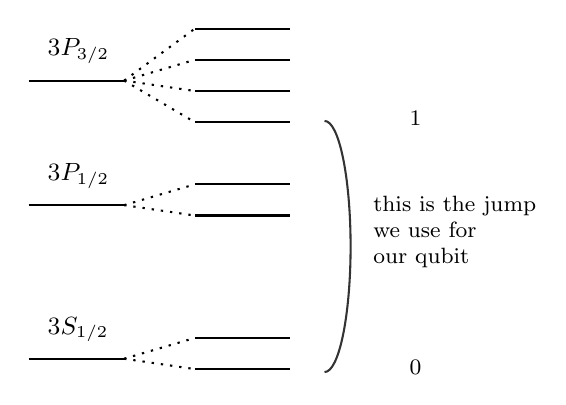
\begin{tikzpicture}[x=0.75pt,y=0.75pt,yscale=-1,xscale=1]
%uncomment if require: \path (0,190); %set diagram left start at 0, and has height of 190

%Straight Lines [id:da34059204718825886] 
\draw    (10,35) -- (25.97,35) -- (55.97,35) ;
%Straight Lines [id:da7025516674321846] 
\draw [line width=0.75]    (90,10) -- (105.97,10) -- (135.97,10) ;
%Straight Lines [id:da6658267546162004] 
\draw [line width=0.75]    (90,25) -- (105.97,25) -- (135.97,25) ;
%Straight Lines [id:da4714600148745056] 
\draw [line width=0.75]    (90,40) -- (105.97,40) -- (135.97,40) ;
%Straight Lines [id:da16901485927223803] 
\draw [line width=0.75]    (90,55) -- (105.97,55) -- (135.97,55) ;
%Straight Lines [id:da1939490218190003] 
\draw  [dash pattern={on 0.84pt off 2.51pt}]  (55.97,35) -- (90,10) ;
%Straight Lines [id:da5816163902648138] 
\draw  [dash pattern={on 0.84pt off 2.51pt}]  (55.97,35) -- (90,25) ;
%Straight Lines [id:da610618410737474] 
\draw  [dash pattern={on 0.84pt off 2.51pt}]  (55.97,35) -- (90,55) ;
%Straight Lines [id:da9192678870004782] 
\draw  [dash pattern={on 0.84pt off 2.51pt}]  (55.97,35) -- (90,40) ;
%Straight Lines [id:da9929664262930785] 
\draw    (10,95) -- (25.97,95) -- (55.97,95) ;
%Straight Lines [id:da5065393969849171] 
\draw [line width=0.75]    (90,85) -- (105.97,85) -- (135.97,85) ;
%Straight Lines [id:da5118777096116628] 
\draw [line width=0.75]    (90,100) -- (105.97,100) -- (135.97,100) ;
%Straight Lines [id:da5444849394573406] 
\draw  [dash pattern={on 0.84pt off 2.51pt}]  (55.97,95) -- (90,85) ;
%Straight Lines [id:da7828314169133617] 
\draw  [dash pattern={on 0.84pt off 2.51pt}]  (55.97,95) -- (90,100) ;
%Straight Lines [id:da31797955021255253] 
\draw    (10,169) -- (25.97,169) -- (55.97,169) ;
%Straight Lines [id:da7584898264764725] 
\draw [line width=0.75]    (90,159) -- (105.97,159) -- (135.97,159) ;
%Straight Lines [id:da14741105203655902] 
\draw [line width=0.75]    (90,174) -- (105.97,174) -- (135.97,174) ;
%Straight Lines [id:da2103499876371232] 
\draw  [dash pattern={on 0.84pt off 2.51pt}]  (55.97,169) -- (90,159) ;
%Straight Lines [id:da47885891493979593] 
\draw  [dash pattern={on 0.84pt off 2.51pt}]  (55.97,169) -- (90,174) ;
%Shape: Arc [id:dp22001354960228459] 
\draw  [draw opacity=0] (152.54,54.43) .. controls (152.54,54.43) and (152.54,54.43) .. (152.54,54.43) .. controls (159.46,54.43) and (165.08,81.51) .. (165.08,114.93) .. controls (165.08,148.34) and (159.46,175.43) .. (152.54,175.43) -- (152.54,114.93) -- cycle ; \draw [color={rgb, 255:red, 51; green, 51; blue, 51 }  ,draw opacity=1 ]   (152.54,54.43) .. controls (159.46,54.43) and (165.08,81.51) .. (165.08,114.93) .. controls (165.08,148.34) and (159.46,175.43) .. (152.54,175.43) ;  

% Text Node
\draw (17.67,13.4) node [anchor=north west][inner sep=0.75pt]  [font=\small]  {$3P_{3/2}$};
% Text Node
\draw (17.67,73.4) node [anchor=north west][inner sep=0.75pt]  [font=\small]  {$3P_{1/2}$};
% Text Node
\draw (17.67,147.4) node [anchor=north west][inner sep=0.75pt]  [font=\small]  {$3S_{1/2}$};
% Text Node
\draw (174.5,89) node [anchor=north west][inner sep=0.75pt]  [font=\footnotesize] [align=left] {this is the jump\\we use for\\our qubit};
% Text Node
\draw (192,48.4) node [anchor=north west][inner sep=0.75pt]  [font=\footnotesize]  {$\ket{1}$};
% Text Node
\draw (192,168.4) node [anchor=north west][inner sep=0.75pt]  [font=\footnotesize]  {$\ket{0}$};


\end{tikzpicture}

\end{center}
\end{tcolorbox}

\subsubsection{Selection rules}

A final comment is about the selection rules that must be changed. The Wigner-Eckart theorem allows to find the new selection rules: 
\begin{align}
     \Delta j &= 0, \pm 1 \quad \text{except when}\quad j=j'=0 \qquad \text{and} \qquad \Delta j_z &= 0, \pm 1 
\end{align}

